% TU Delft Beamer template
% Author: Maarten Abbink
% Delft University of Technology
% March 2014
% Version 2.0
% Based on original version 1.0 of Carl Schneider
\documentclass{beamer}
\usepackage[english]{babel}
\usepackage{calc}
\usepackage[absolute,overlay]{textpos}
\usepackage{minted}
\mode<presentation>{\usetheme{tud}}

\title[A type system for dynamic instances]{A type system for dynamic instances}
%\subtitle
\institute[TU Delft]{Delft University of Technology}
\author{Albert ten Napel}
\date{\today}

% Insert frame before each subsection (requires 2 latex runs)
\AtBeginSubsection[] {
	\begin{frame}<beamer>\frametitle{\titleSubsec}
		\tableofcontents[currentsection,currentsubsection]  % Generation of the Table of Contents
	\end{frame}
}
% Define the title of each inserted pre-subsection frame
\newcommand*\titleSubsec{Next Subsection}
% Define the title of the "Table of Contents" frame
\newcommand*\titleTOC{Outline}

% define a symbol which can be removed if you don't need it
\newcommand{\field}[1]{\mathbb{#1}}
\newcommand{\Zset}{\field{Z}}

\begin{document}

{
% remove the next line if you don't want a background image
\usebackgroundtemplate{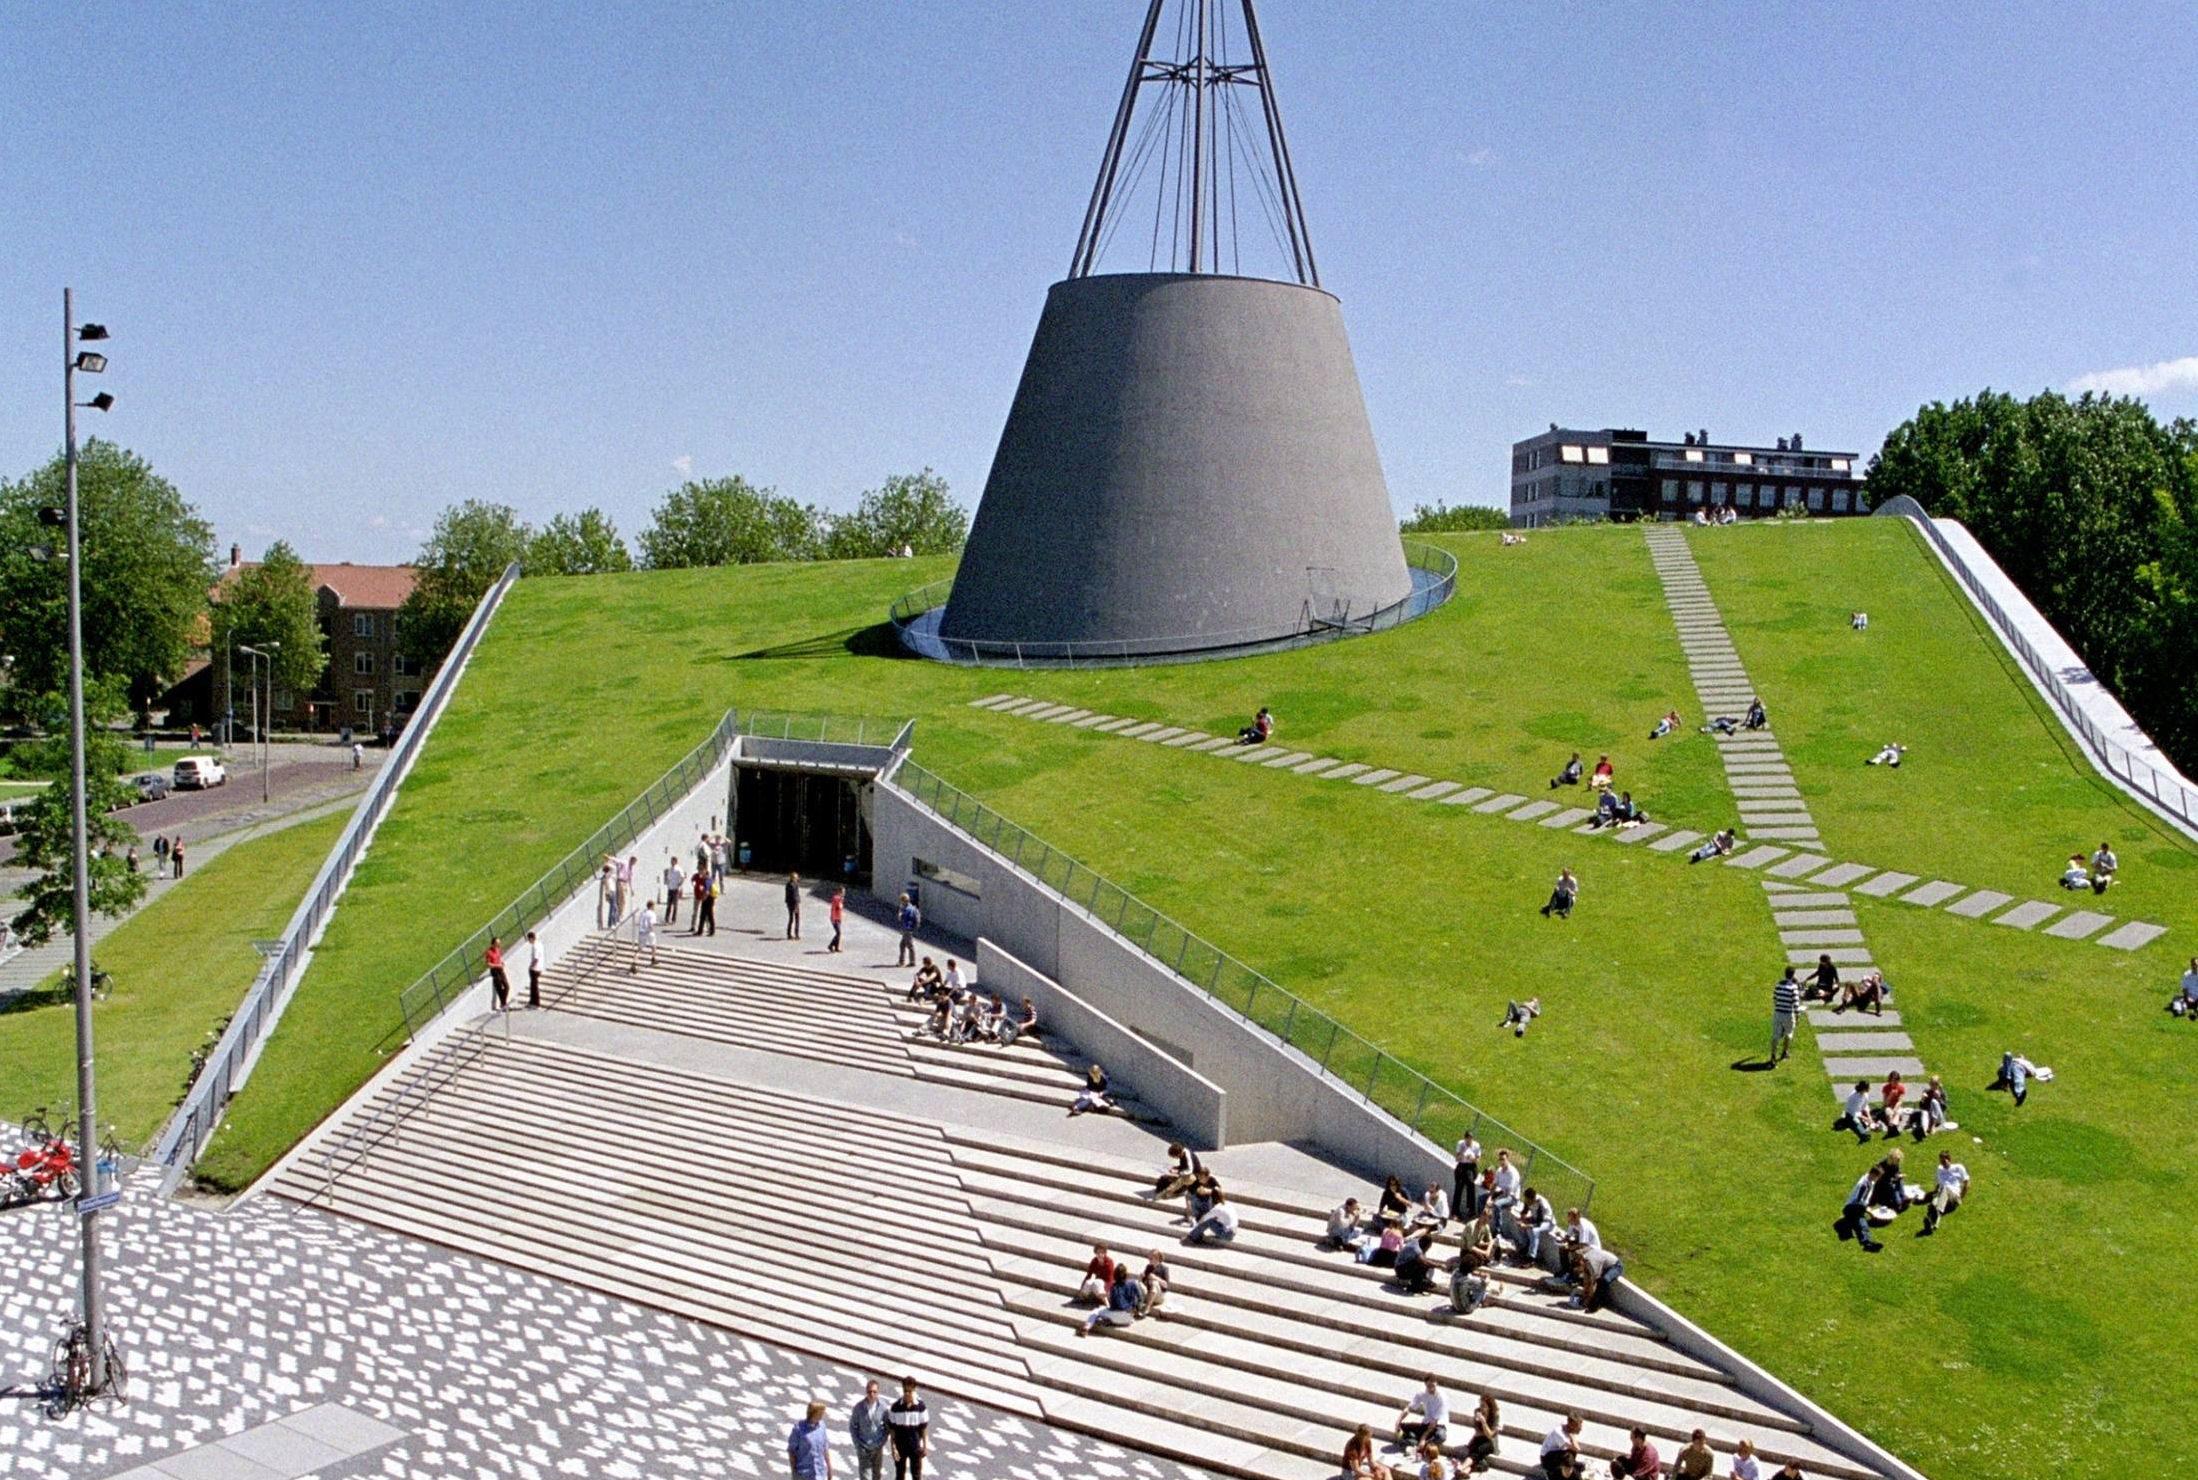
\includegraphics[width=\paperwidth,height=\paperheight]{images/background-titlepage.jpg}}%
\setbeamertemplate{footline}{\usebeamertemplate*{minimal footline}}
\frame{\titlepage}
}

{\setbeamertemplate{footline}{\usebeamertemplate*{minimal footline}}
\begin{frame}\frametitle{\titleTOC}
	\tableofcontents
\end{frame}
}

\section{What are effects}

\begin{frame}[fragile]\frametitle{Effects}
	\begin{example}
		\begin{minted}{haskell}
x = 10
5 - 6
		\end{minted}
	\end{example}
\end{frame}

\section{Algebraic effects and handlers}

\section{Miro}

\begin{frame}[fragile]\frametitle{Miro - Creating instances}
\begin{example}
\begin{minted}[tabsize=2]{haskell}
ref : forall s. Int -> (Inst s State)!{s}
ref [s] v =
	new State@s {
		get () k -> \st -> k st st
		put st' k -> \st -> k () st'
		return x -> \st -> return x
		finally f -> f v
	} as x in return x
\end{minted}
\end{example}
\end{frame}

\begin{frame}[fragile]\frametitle{Miro - Using instances}
\begin{example}
\begin{minted}[tabsize=2]{haskell}
postInc : forall s. Inst s State -> Int!{s}
postInc [s] inst =
	x <- inst#get();
	inst#put(x + 1);
	return x
\end{minted}
\end{example}
\end{frame}

\begin{frame}[fragile]\frametitle{Miro - Running instances}
\begin{example}
\begin{minted}[tabsize=2]{haskell}
result : Int!{}
result =
	runscope(s1 ->
		r1 <- ref [s1] 10;
		runscope(s2 ->
			r2 <- ref [s2] 20;
			x <- postInc [s2] r2;
			r1#put(x);
			return x);
		y <- r1#get ();
		return y) -- result is 20
\end{minted}
\end{example}
\end{frame}

\section{Semantics}

\section{Type system}

\subsection{Type safety}

\section{Future work}

\section{Questions}

\end{document}
